\chapter{Diagram} \label{appendix:diagram}

% IKKE SLETT VIL HA DENNE SOM EKSEMPEL
%\begin{figure}[ht]
% 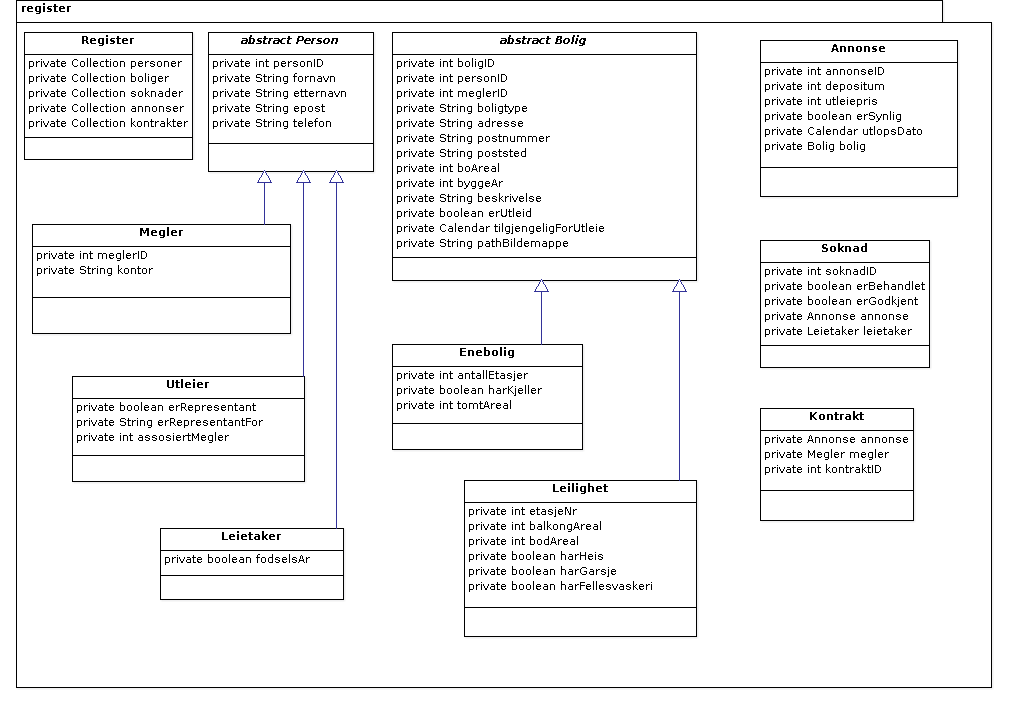
\includegraphics[angle=90 ,width=\textwidth,height=\textheight,keepaspectratio]{./img/appendix/diagram/klassestruktur_uml.png}
% \caption{Innledende UML diagram. brukt for generering av grunnleggende klasser.}
% %Her kommer en kabel for kryssreferering i teksten til figuren
% \label{fig:uml_diag}
%\end{figure}

\begin{figure}[ht]
\begin{center}
 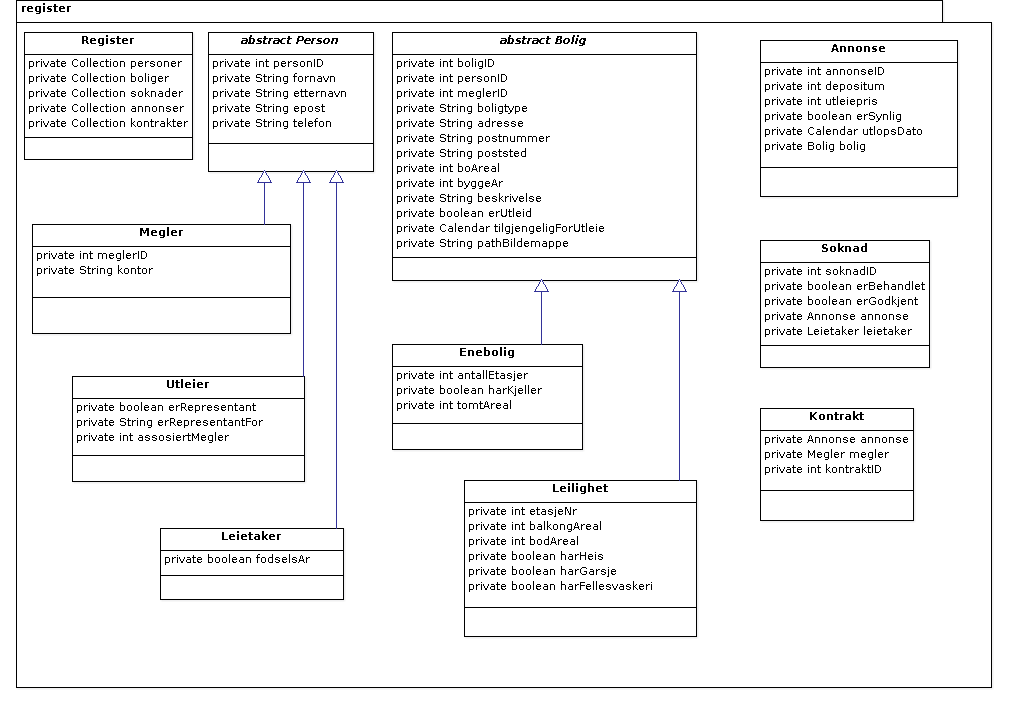
\includegraphics[angle=90, height=21cm]{./img/appendix/diagram/klassestruktur_uml.png}
 \caption[UML]{Innledende UML diagram. brukt for generering av grunnleggende klasser.}
 %Her kommer en kabel for kryssreferering i teksten til figuren
 \label{fig:uml_diag}
 \end{center}
\end{figure}


\begin{figure}[ht]
 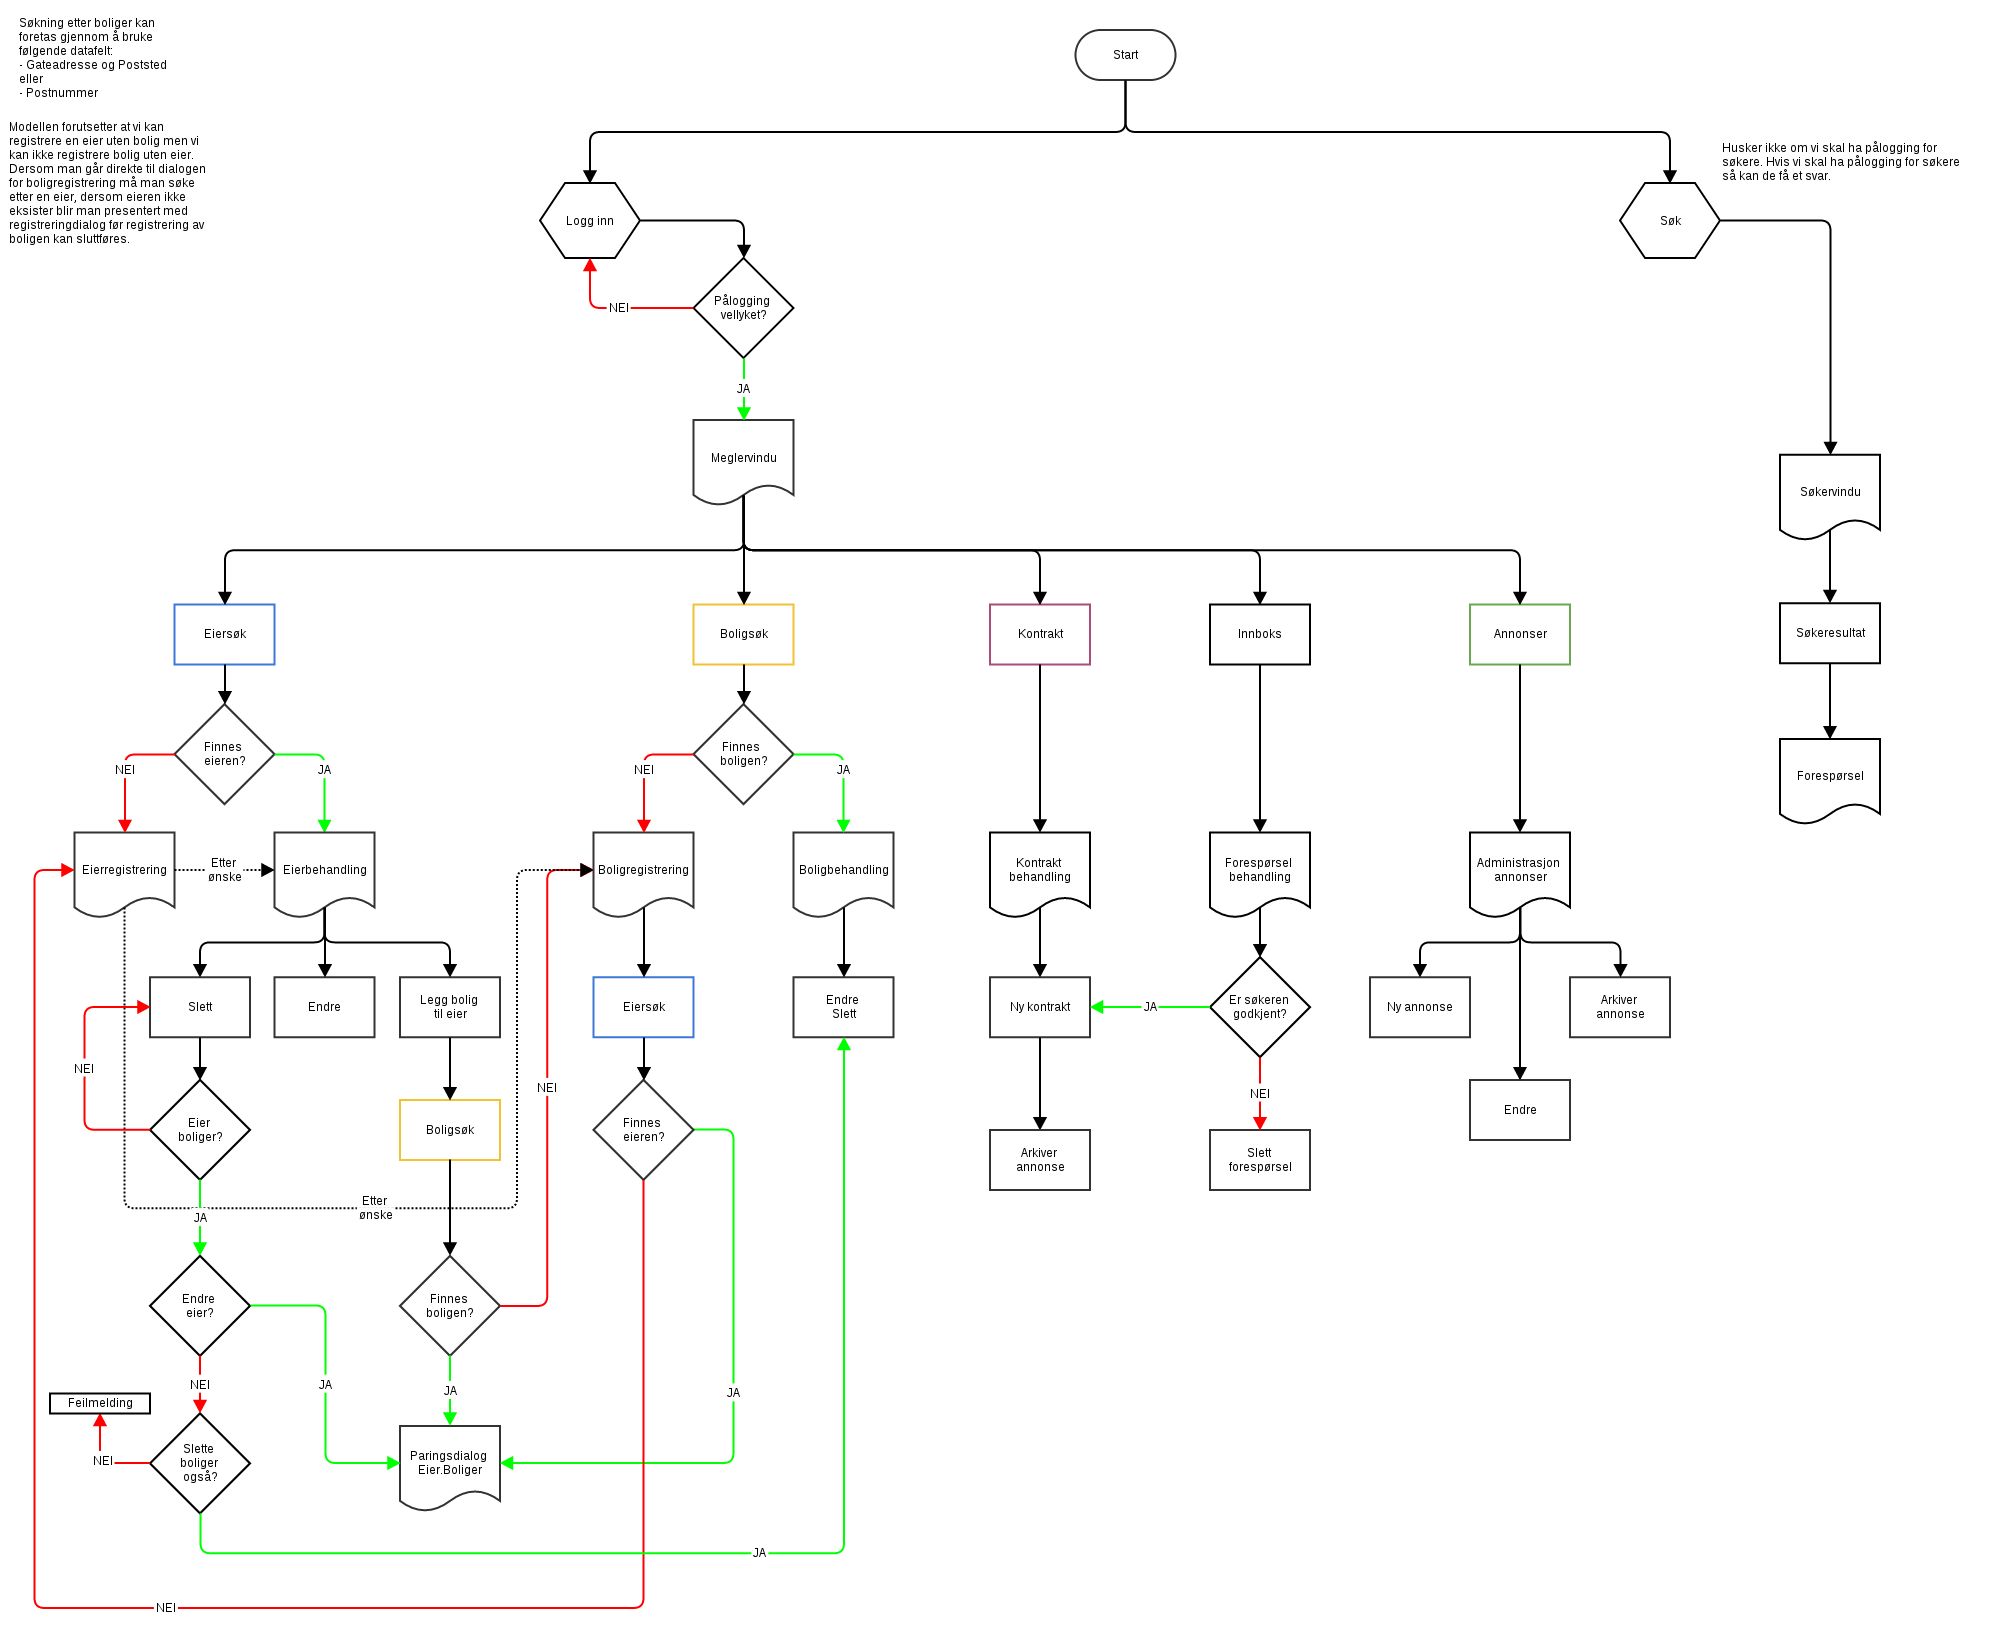
\includegraphics[angle=90 ,width=\textwidth,height=\textheight,keepaspectratio]{./img/appendix/diagram/user_case.png}
 \caption[Brukercase]{Flyt diagram over mulig user case som kan foretas i brukergrensesnittet.}
 %Her kommer en kabel for kryssreferering i teksten til figuren
 \label{fig:user_case}
\end{figure}



\begin{figure}[ht]
\begin{center}
 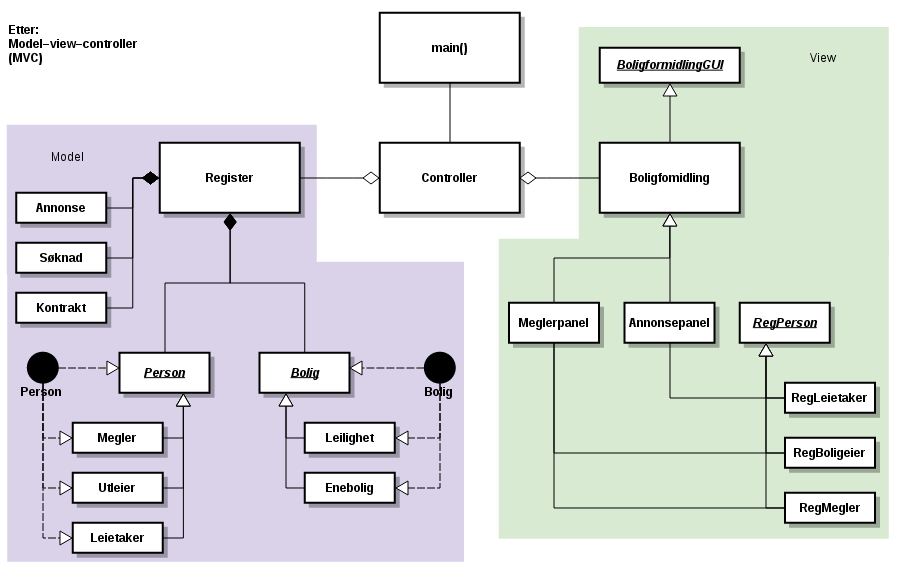
\includegraphics[angle=90, height=21cm]{./img/appendix/diagram/moduler_og_relasjoner.png}
 \caption[MVC - første utkast]{Innledende diagram over planlagt MVC arkitektur i programmet.}
 %Her kommer en kabel for kryssreferering i teksten til figuren
 \label{fig:mvc_innledende}
  \end{center}
\end{figure}

\begin{figure}[ht]
\begin{center}
 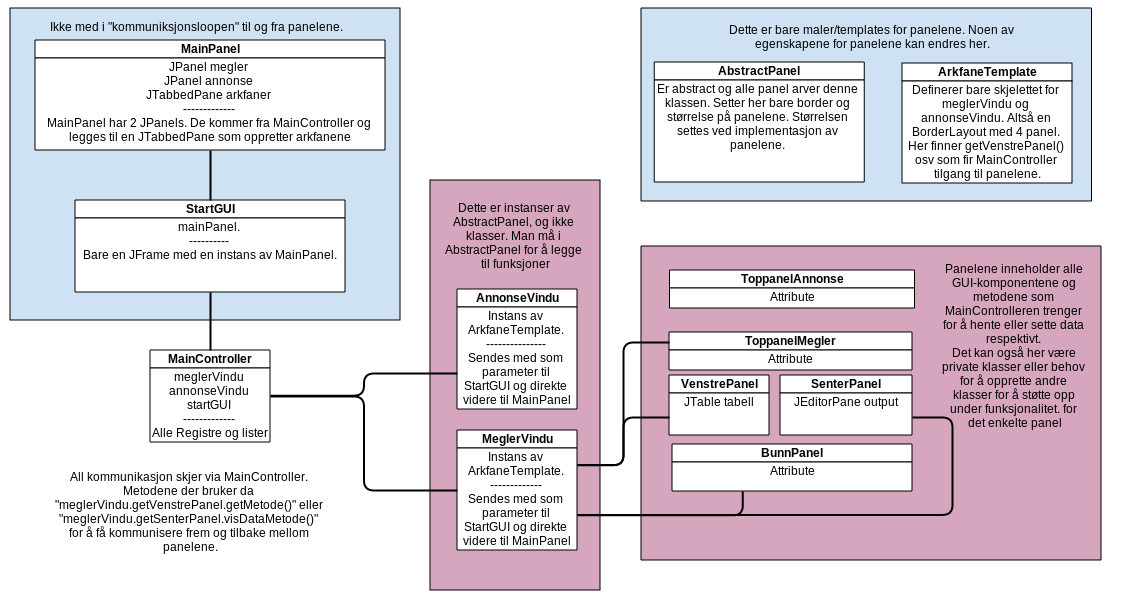
\includegraphics[angle=90, height=21cm]{./img/appendix/diagram/controller_og_gui.png}
 \caption[Kontroller og GUI]{Flytdiagram over kontroller og GUI klasser.}
 %Her kommer en kabel for kryssreferering i teksten til figuren
 \label{fig:kontroller_og_gui}
 \end{center}
\end{figure}


\begin{figure}[ht]
\begin{center}
 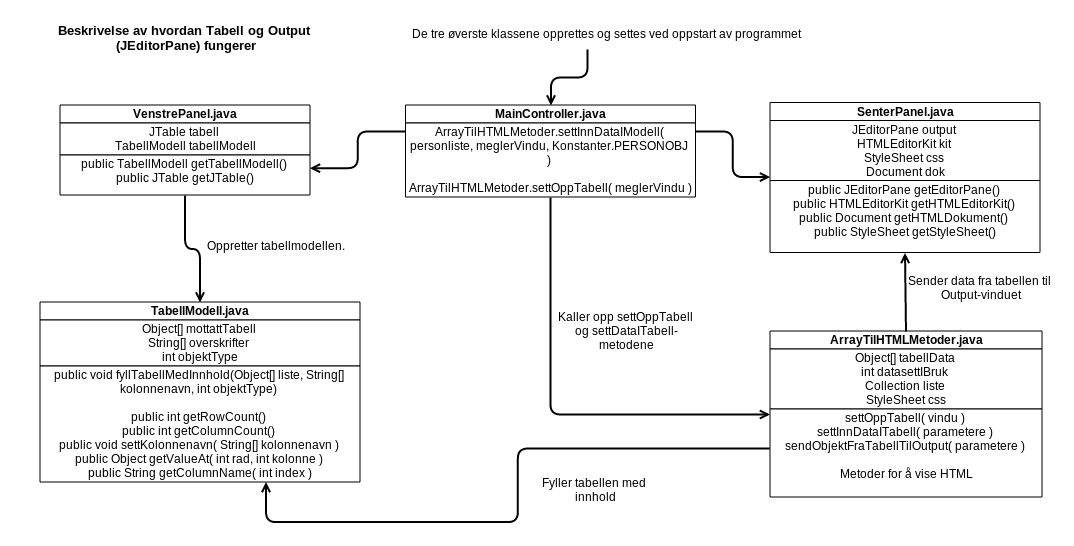
\includegraphics[angle=90 , height=21cm]{./img/appendix/diagram/tabell_og_output.png}
 \caption[Tabellmodell og output]{Flytdiagram over tabellmodell og output.}
 %Her kommer en kabel for kryssreferering i teksten til figuren
 \label{fig:tabell_og_output}
  \end{center}
\end{figure}